The conversational workflow is instantiated through a dynamic, state-driven interaction model that coordinates between user inputs and recommendation logic, all defined in a \texttt{HybridCRSWorkflow} module. It maintains context, tracks preferences, and integrates multi-source recommendations. This interaction happens across discrete steps, each encapsulated as an event in the graph-based conversational controller, as described previously in Figure~\ref{FIG:EVENT_WORKFLOW}. The implementation of the conversational process can be broken down in several steps, as depicted in the high-level workflow diagram in Figure~\ref{FIG:HYBRID_WORKFLOW}.

\begin{figure}[High-Level Conversational Workflow]{FIG:HYBRID_WORKFLOW}{A high-level diagram of the Hybrid Conversational Recommendation Workflow.}
    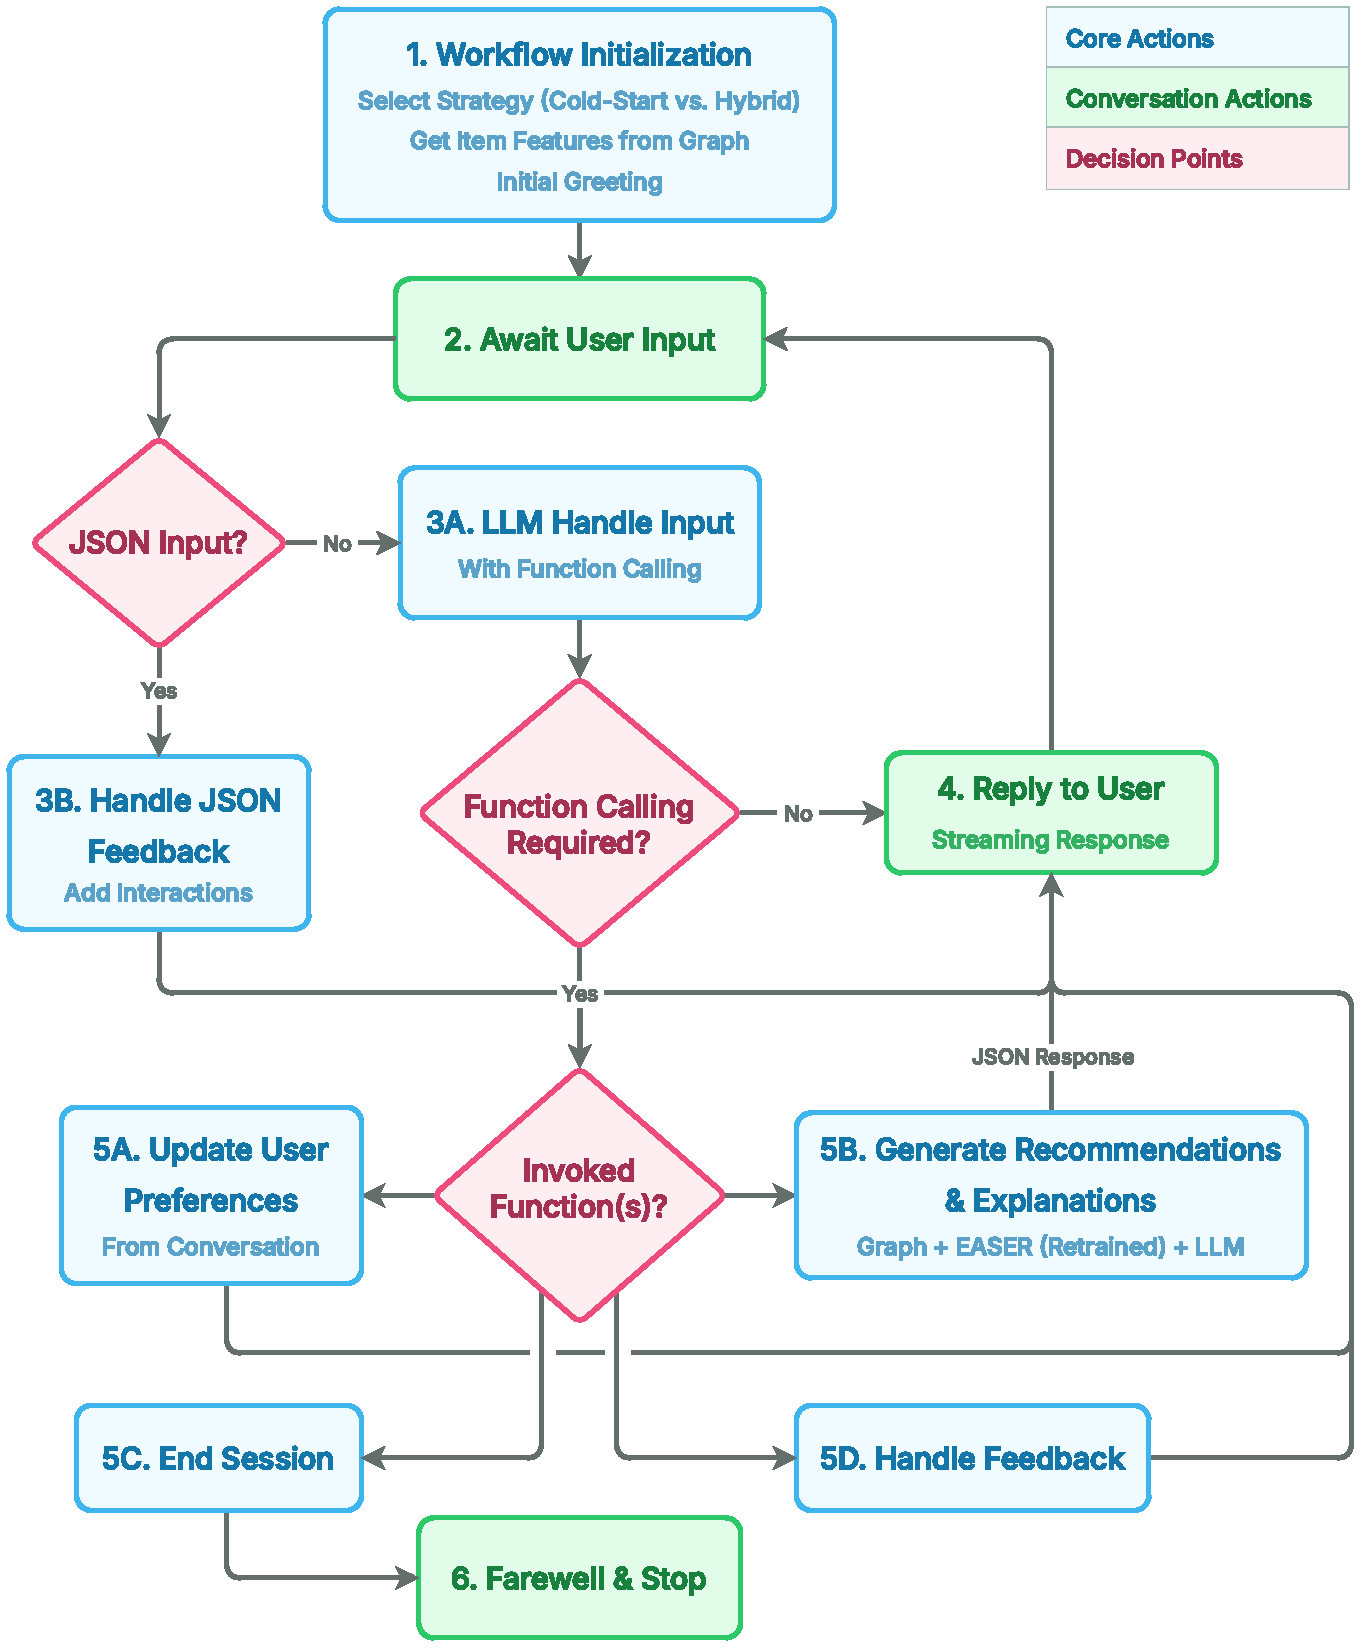
\includegraphics[width=\textwidth]{hybrid_crs_workflow.pdf}
\end{figure}


\begin{compactenum}
    \item \textbf{Session Initialization}:
    \begin{compactitem}
        \item The agent begins by extracting the feature schema from a structured item graph (e.g., \textit{name}, \textit{category}, \textit{rating}).
        \item The system dynamically determines user status (\texttt{cold-start} vs. \texttt{expert-enabled}) from interaction count.
        \item A memory buffer is initialized with an introductory prompt, which includes the dataset description. 
        \item The agent introduces itself and initiates the first user interaction.
    \end{compactitem}

    \item \textbf{User Turn and Input Processing}:
    \begin{compactitem}
        \item Upon receiving a user utterance, the memory buffer logs the interaction history.
        \item The agent evaluates whether the input contains structured feedback (e.g., explicit ratings) or free-text natural language.
        \item Based on this classification, different response paths are followed---either to register feedback or to query further preferences.
    \end{compactitem}

    \item \textbf{Tool Invocation and Autonomous Action}:
    \begin{compactitem}
        \item The agent determines---without hardcoded rules---whether a tool should be invoked.
        \item Tool options include preference updates, recommendation requests, feedback processing, or terminating the session.
        \item Each tool is dynamically chosen based on context and invoked with parameters derived from the ongoing dialogue.
    \end{compactitem}

    \item \textbf{Preference Elicitation and Correction}:
    \begin{compactitem}
        \item When a preference is expressed, it is validated against the known schema of item features.
        \item If a mismatch is detected (e.g., \textit{``comedyish''} instead of \textit{``comedy''}), the agent attempts to infer the correct canonical value.
        \item Preferences are stored incrementally in a structured user profile that supports categorical, numerical, and token-based types.
    \end{compactitem}

    \item \textbf{Recommendation Generation}:
    \begin{compactitem}
        \item When sufficient information has been gathered, the agent requests personalized recommendations.
        \item For new users, contextual reasoning is applied using item-attribute filtering from the graph-based backend.
        \item For existing users, a hybrid strategy is adopted---merging graph-based reasoning (contextual recommendations \& \acl{cf}) and the expert \texttt{EASER} model.
        \item The top results are merged and presented with natural language explanations.
    \end{compactitem}

    \item \textbf{Explanation Generation}:
    \begin{compactitem}
        \item Structured explanation facts from the graph-based model (e.g., shared categories, popularity) are aggregated.
        \item These are then paraphrased into a coherent, user-facing justification by the agent.
        \item The final output is delivered as a fluent paragraph that contextualizes each recommended item.
    \end{compactitem}

    \item \textbf{Feedback Collection and Adaptation}:
    \begin{compactitem}
        \item Users may respond to recommendations with explicit (e.g., JSON ratings) or implicit feedback (e.g., \textit{``I liked the first one''}).
        \item The agent interprets this feedback, updates the user profile, inserts user-item interactions into the graph, and into the interaction dataset in disk.
    \end{compactitem}

    \item \textbf{Session Termination}:
    \begin{compactitem}
        \item If the user signals completion (e.g., \textit{``that's all for now''}), the agent invokes a termination tool.
        \item A closing message is generated and the session is finalized.
    \end{compactitem}
\end{compactenum}

The agent's operation within this workflow is entirely asynchronous and stateful. Each event transition is informed by the user's evolving preferences and previous interactions, enabling a fluid, mixed-initiative dialogue that adapts to diverse user needs. As the session progresses, the agent alternates seamlessly between eliciting preferences, recommending items, and incorporating feedback---all while preserving a coherent conversation thread.
